%!TEX root = ttc14-fixml.tex

\section{\SIGMA Overview}
\label{sec:SigmaOverview}

\SIGMA DSLs are embedded in Scala~\cite{Odersky2004}, a statically typed production-ready General-Purpose Language (GPL) that supports both object-oriented and functional styles of programming.
Scala uses type inference to combine static type safety with a \emph{``look and feel''} close to dynamically typed languages.
It is interoperable with Java and has been designed to host internal DSLs~\cite{Chafi2010}.
Furthermore, it is supported by the major integrated development environments.

A typical way of embedding a shallow DSL into Scala is by designing a library that allows one to write fragments of code with domain-specific syntax.
These fragments are woven within Scala own syntax so that it appears different~\cite{Dubochet2011}.
Next to Scala flexible syntax (\Eg omitting semicolons and dots in method invocations, infix operator syntax for method calls, etc.), it has a number of features simplifying DSL embedding such as
%
\begin{inparaitem}[]
  \item implicit type conversions allowing one to extend existing types with new methods,
  \item mixin-class composition (\Ie reusing a partial class definition in a new class)~\cite{Odersky2004}, and 
  \item lifting static source information with implicit resolutions to customize error messages in terms of the domain-specific extensions using annotations~\cite{Moors2012}.
\end{inparaitem}

\begin{figure}[h!bt]
  \centering
  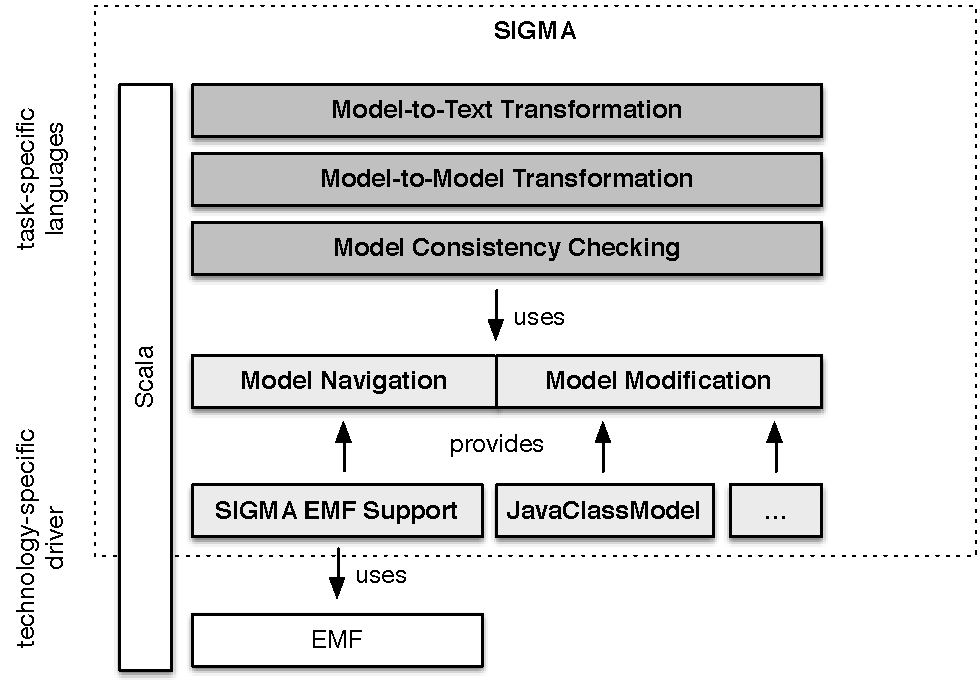
\includegraphics[width=10cm]{figures/SigmaOverview.pdf}
  \caption{Sigma EMF to Scala Support}
  \label{fig:SigmaStack}
\end{figure}

Figure~\ref{fig:SigmaStack} depicts the general organization of the \SIGMA DSLs~\cite{Krikava2014}.
The use of EMF models in \SIGMA is facilitated by a dedicated support layer that underneath uses the default EMF generated Java classes and the EMF API.
This layer provides a convenient model navigation and modification support forming a common infrastructure for the task-specific internal DSLs.
While \SIGMA targets the EMF platform, other meta-modeling platforms could be used as well.
In Section~\ref{sec:Extension3} we will show how to create a support for a Java class model.